\chapter{PACORA Implementation in a Manycore Operating System}\label{tess_design_ch}
In this chapter, we present our implementation of \pacora in \tess OS, a manycore research operating system \cite{tess_resource, tess, tess_dac, tess_audio, tess_gui}.  We give an overview of \tess and why we chose it for our implementation.  We then discuss the details for building RTFs online in the operating system.  Finally, we present our implementation of the resource allocator using an ADMM optimization method.



\section{Motivation}

We believe \pacora is applicable to many resource-allocation
scenarios from cloud computing to distributed embedded systems. For our initial prototype, we chose to study
\pacora implemented in a general-purpose operating system for client
systems, because we believe this scenario has some of the most
difficult resource allocation challenges: a constantly changing
application mix requiring low overhead and fast response times, shared
resources that create more interference among the applications, and
platforms that are too diverse to allow \emph{a priori} performance
prediction.

To evaluate \pacora's ability to make real-time decisions in a real operating system, we implemented it in an in-house research operating system, \tess. We chose to implement in \tess rather than Linux for three reasons:
 \begin{enumerate}\itemsep0pt \parskip0pt \parsep5pt
\item \tess separates resource allocation from scheduling, so is
  closer to the OS architecture assumed by \pacora
\item \tess allows resource revocation, enabling \pacora to dynamically reallocate resources
\item \tess implements additional resource partitioning mechanisms,
  letting \pacora manage  more resource types
\end{enumerate}

 Further, modifying a full-fledged production OS such as Linux to investigate new resources management schemas is complex and
 requires more implementation effort than developing for \tess's resource-centric OS\footnote{For example, the Earliest
 Deadline First (EDF) scheduler in \tess is only 800 lines of user-space code, contained in four files.  By contrast, support for
 EDF in Linux requires kernel modifications and substantially more code: the best-known EDF kernel patch for Linux, SCHED\_DEADLINE, has over 3500 modified lines in over 50 files.}.
We use the \tess implementation to test our implementations of the algorithms, measure the overhead and reaction times, and illustrate \pacora's ability to work in a real system. 

\section{\tess Overview}

This section briefly describes the key components of \tess OS~\cite{tess,tess_resource,tess_dac,tess_audio, tess_gui}.
The \tess kernel is a thin, hypervisor-like layer that provides support
for dynamic resource management.  It implements cell along with interfaces for user-level scheduling, resource
adaptation, and cell composition.  \tess currently runs on x86 hardware
platforms (\emph{e.g.,} with Intel's Sandy Bridge CPUs). 


\subsection{Cells}\label{sec:cell-model}

In \tess, resources are distributed to QoS domains called
\emph{cells}, which are explicitly parallel, light-weight, performance-isolated containers
with guaranteed, user-level access to resources. The software running within each cell has full
user-level control of the cell's resources.

\begin{figure}[tp]
%\vspace*{-0.2in}
\centering
%\rule{4cm}{3cm}
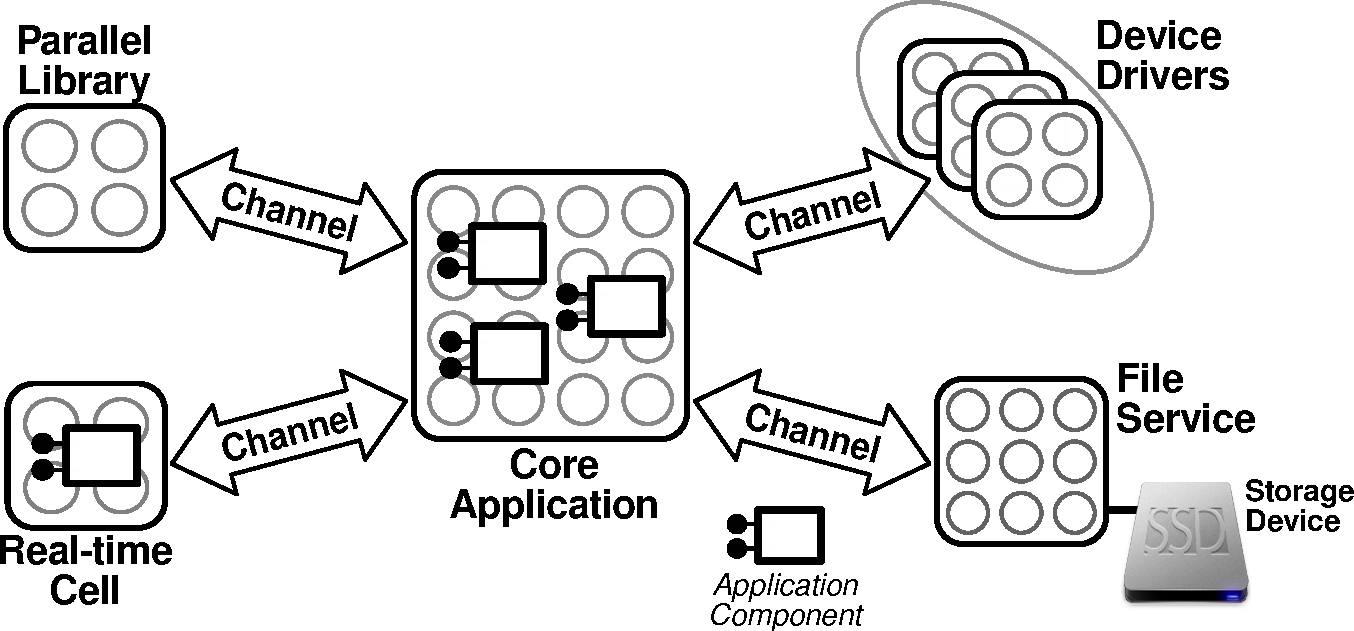
\includegraphics[width=1.0\columnwidth]{Figures/app-split-into-cells.pdf}
%\vspace*{-0.4in}
\caption{
Applications in \tess are created as sets of interacting components
hosted in different cells that communicate over channels.
Standard OS services (\eg the file service) are also hosted in cells and
accessed via channels.
}
\label{fig:app-split-into-cells}
%\vspace*{-0.15in}
\end{figure}

As depicted in Figure~\ref{fig:app-split-into-cells}, applications
in \tess are created by composing cells via \emph{channels}, which
provide fast, user-level asynchronous message-passing between cells.
Applications can then be split into performance-incompatible and
mutually distrusting cells with controlled communication. 


\tess OS implements cells on x86 platforms by partitioning resources
using \emph{space-time partitioning}~\cite{rushby99,lei03}, 
a multiplexing technique that divides the hardware into a sequence of
simultaneously-resident spatial partitions. 
Cores and other resources are
\textit{gang-scheduled}~\cite{gangsched1982,gangschedpatent}, so
cells provide to their hosted applications an environment that is very
similar to a dedicated machine.

\subsection{Resources and Services} \label{sec:soa} 
Partitionable resources include CPU cores, memory pages, and guaranteed
fractional services from other cells (\emph{e.g.,} a throughput reservation of 150~Mbps
from the network service).  
They may also include cache slices, portions of memory bandwidth, and fractions
of the energy budget, when hardware support is available
\cite{akesson07,lee08memqos,paolieri09,sanchez11}.

\tess also creates \emph{service cells} to encapsulate user-level device drivers and control devices.
Each service can thus arbitrate access to its
enclosed devices to offer service guarantees to
other cells. \tess treats the services
offered by the service cells as additional resources to be allocated to applications.

\tess currently has two such service cells implemented:
the \emph{Network Service}, which provides access to network adapters and
guarantees that the data flows are processed with the agreed levels of
throughput; and the \emph{GUI Service}, which provides a windowing system with
response-time guarantees for visual applications.  


\subsection{Resource Management and Scheduling} 

\begin{figure}[t]
\centering
%\rule{4cm}{3cm}
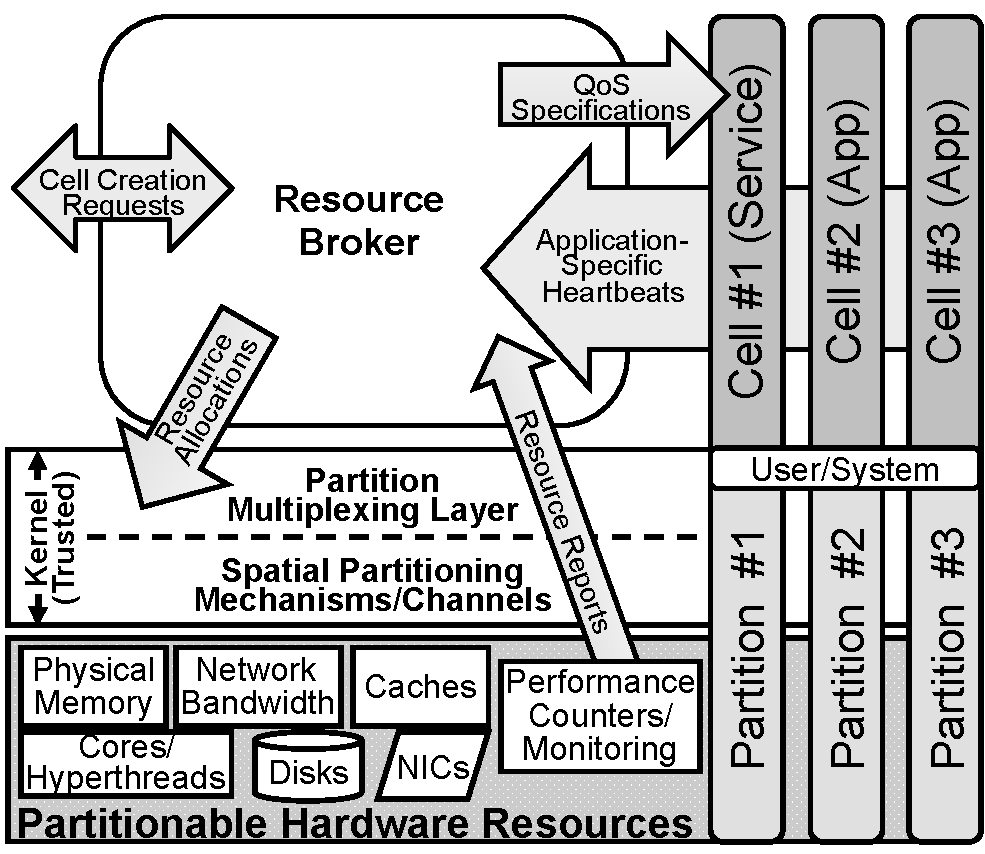
\includegraphics[width=0.885\linewidth]{Figures/NewPolicyFig-Tess}
%\vspace*{-0.1in}
\caption{
The \tess kernel implements \emph{cells} through \emph{spatial-partitioning}.
The \emph{Resource Broker} redistributes resources after consulting application-specific
\emph{heartbeats} and system-wide \emph{resource reports}.
}
\label{fig:tess-arch}
%\vspace*{-0.175in}
\end{figure}

\tess uses \emph{Two-level scheduling}~\cite{leiner07,ober08} %,tess10} 
to separate global decisions about allocation of resources \emph{to}
cells (\emph{first level}) from application-specific usage of resources
\emph{within} cells (\emph{second level}). 
Resource allocation occurs at a coarse time scale to allow time for cell scheduling decisions to become effective.

\subsubsection{Scheduling}
Scheduling within cells functions purely at the user-level, as
close to the \emph{bare metal} as possible, improving efficiency and
eliminating unpredictable OS interference.  \tess provides a framework for preemptive
scheduling, called \emph{Pulse}, enables customization and support for a wide
variety of application-specific runtimes and schedulers without
kernel-level modifications. 
The user-level runtime within each cell can be tuned for a specific
application or application domain with a custom scheduling algorithm.
Using Pulse, \tess provides pre-canned
implementations for TBB~\cite{tbb07} and a number of scheduling algorithms,
including Global Round Robin (GRR), Earliest Deadline First
(EDF), and Speed Balancing~\cite{juggle2013}.  
 
Pulse provides support for revoking resource from schedulers. If a core is removed, Pulse's auxiliary scheduler runs the cell's outstanding scheduler contexts in
a globally \emph{cooperative}, Round Robin manner; \ie a scheduler context runs
until it either completes and transitions into an application context, or yields
into Pulse, allowing other contexts to run. Additionally, the Pulse API provides callbacks to notify schedulers when the number of available cores
changes, enabling resource-aware scheduling. 

\subsubsection{Adaptive Resource Allocation} \label{sec:rsc-alloc}

Global resource allocation in Tessellation is performed by the \emph{Resource Broker}, as
shown in Figure~\ref{fig:tess-arch}. The Broker assigns 
resources to cells and communicates its allocation decisions to the kernel
and services for enforcement.  It reallocates resources,
for example, when a cell starts or finishes or when a cell significantly
changes performance.  The Broker can periodically adjust allocations; the
reallocation frequency provides a tradeoff between adaptability (to
changes in state) and stability (of user-level scheduling).

Rather than implementing a single policy, the Broker is resource allocation framework that supports
rapid development and testing of new allocation policies. We've implemented \pacora as a resource allocation policy inside the Resource Broker.
 
\section{\pacora in \tess}

\begin{figure}[t]
\centering
%\rule{4cm}{3cm}
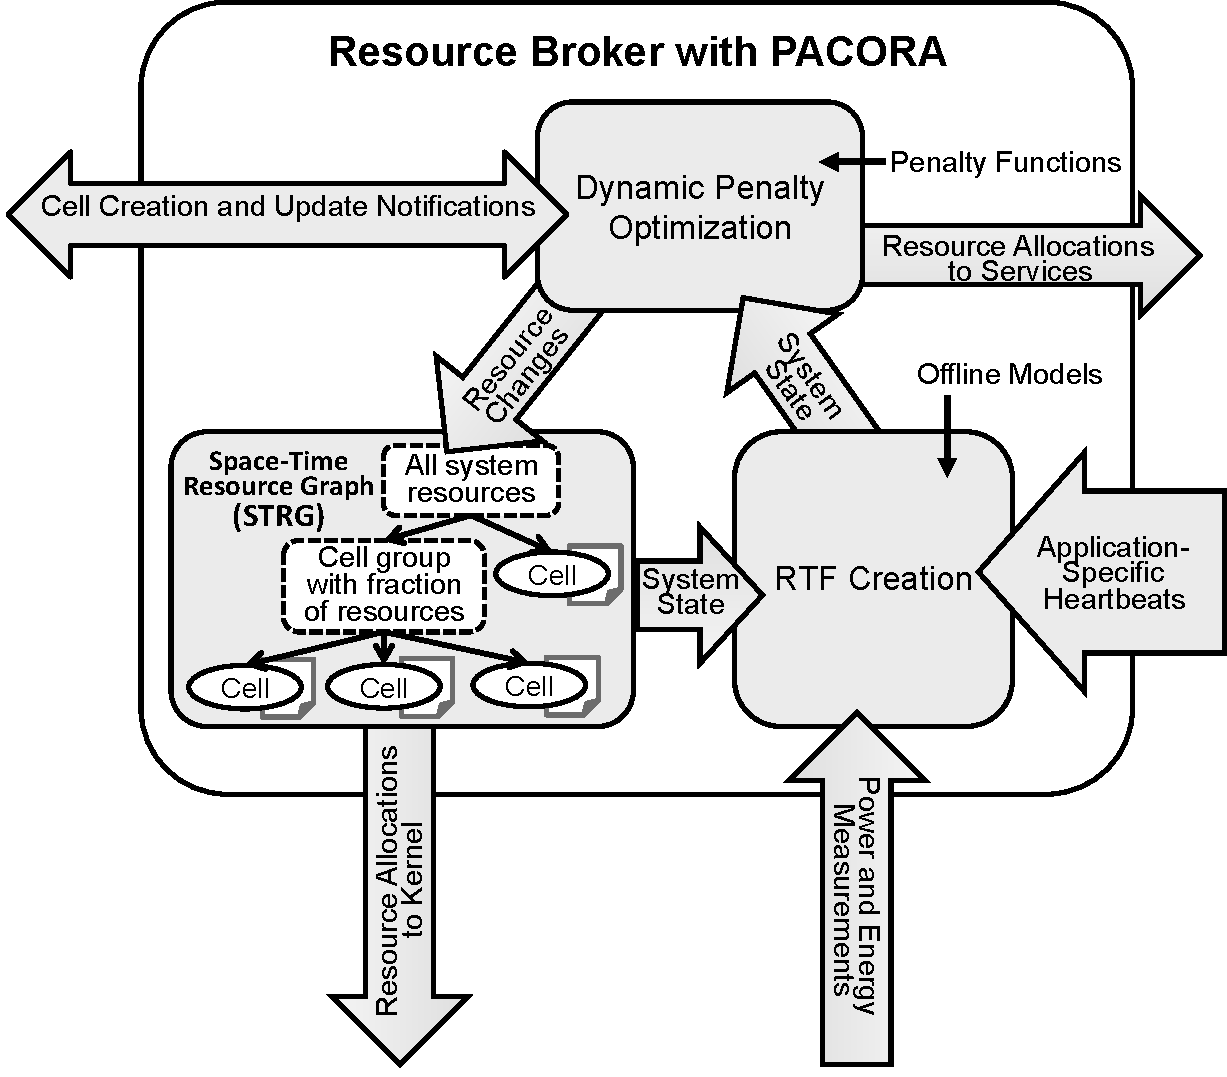
\includegraphics[width=0.885\linewidth]{Figures/pacora-in-tess}
%\vspace*{-0.1in}
\caption{
Overview of \pacora implementation in \tess.  \pacora leverages the existing Resource Broker interfaces to communicate with the cells, services, and kernel.  The RTF Creation and Dynamic Penalty Optimization modules contain \pacora's model creation and resource allocation functions.
}
\label{fig:pacora-in-tess}
%\vspace*{-0.175in}
\end{figure}

In this section, we provide details of \pacora's implementation in \tess's Resource Broker. Figure~\ref{fig:pacora-in-tess} shows the design. The Resource Broker runs in its own cell and communicates with applications and services through channels. \pacora leverages the existing Resource Broker interfaces to communicate with the cells, services, and kernel.  The RTF Creation and Dynamic Penalty Optimization modules contain \pacora's model creation and resource allocation functions and are described in Sections~\ref{rtf_creation} and~\ref{dyn_opt} respectively.

\subsection{Cell Creation}

When a cell is started, it opens its own channel with the Resource Broker and sends a cell creation message to register.
The registration message contains the deadline and slope for \pacora's penalty function and optionally, a starting RTF model.  The message format is shown below.

\texttt{register\_cell(...)}


Ideally, penalty functions would be inferred by the system or provided by a
more trusted source than the applications themselves.  The simplest approach to implement this functionality in current operating systems would be to use an application's priority as the penalty slope and its interaction class~\cite{interaction_class} for the deadline. However, for our prototype the direct approach was straightforward to implement, and we believe does not detract from the validity of the resource allocation experiments\footnote{For cloud systems, this approach is, in fact, common practice: applications typically provide their resource requirements to the system.}.  


The Resource Broker also provides an interface for cells to update their penalty function or RTF while they are running, which we currently use to change RTF functions when an application changes phase or update the penalty function of application 0 when the computer changes operating mode (\ie from battery to power source).  The message formats for updating RTFs or Penalty Functions are shown below.

\texttt{update\_rtf}

\texttt{update\_pf}

\subsection{Performance and Power Measurement}
Applications report their own measured response times to \pacora by periodically sending performance report messages, called \emph{heartbeats}~\cite{hoffmann2011}.  Messages may contain the value for a single heartbeat or heartbeats may be batched together.  The batch size is configurable, but is bounded by a maximum size, \texttt{MAX\_REPORT\_SIZE}, set by the system.   The code below shows the heartbeat message format.

\texttt{send\_performance\_report}

\pacora uses this information to build RTFs offline or online.  This process is described in Section~\ref{rtf_creation}.  As with the cell creation interface, it would be better for the system to directly measure application heartbeats rather than needing to trust the application's measurements.  However, measuring application-specific heartbeats in a general-purpose way is a challenging problem, and we chose not to address it in this work.  We instead focus exploring the value of resource allocation using application-specific measurements first.  Heartbeat measurement options are discussed further in Section~\ref{discuss}.

\tess provides a system call (show below) for \pacora to directly measure the system energy using the energy counters available on current x86 systems.  \pacora uses this information to build application 0's RTF.

\texttt{measure\_energy\_counter}


\subsection{Resource Allocation}
\pacora periodically optimizes the system penalty and produces resource allocations.  Details of this process are described in Section~\ref{dyn_opt}.  Allocation decisions are communicated to the kernel and services for enforcement.  Updates are sent to the kernel the update\_cells system call, which adjusts the Space-Time Resource Graph.  The system call is shown below.

\texttt{update\_cells(...)}

The Resource Broker has a channel with each service to communicate allocations.  To update an allocation, \pacora sends a QoS Specification message to the service.  These messages are service-specific.  The network service QoS specification message is shown below.

\texttt{update\_NS\_alloc(...)}

The Resource Broker design provides an adjustable reallocation frequency; the reallocation frequency provides a tradeoff
between adaptability (to changes in state) and stability (of user-level
scheduling).  

If \pacora is using offline models then it only makes sense to reallocate resources when a cell starts or finishes or when a cell updates its penalty function or RTF, since those are only points at which the inputs to the optimization change.  The exception to this is if optimization is terminated early for latency reasons, then each successive reallocation would move the allocations closer to optimial\footnote{We found early termination to be unnecessary since the complete optimization runs so quickly.  (This data is shown in Section~\ref{tess_eval}.)}. 

With online modeling reallocation could, in theory, be performed more frequently since the RTF functions can change as a cell runs.  However, the models will only change significantly as a result of an application phase change or application input change and so, in practice, it is similar to the offline modeling case\footnote{In the cloud, RTFs for applications such as web services may also change as a result of the incoming request load and thus require more frequent reallocation.}.

In our experiments (See Section~\ref{tess_eval}), we run \pacora continuously so that we can observe more resource allocation decisions. However, the allocations rarely change outside of the cases described above (\ie cell start/stop or phase/penalty change), so in practice it performs the same (in terms of resulting allocations) as if it were run periodically but with a higher overhead since it occupies at hardware thread for all time instead for only a single optimization at a time. 

\subsection{Application Requirements}
Our \tess implementation of \pacora requires minor modifications to applications\footnote{In addition to the modifications already required for an application to run on \tess}.  First, during the application initialization phase where the cell registers with \tess, a cell creation call must be added to open a channel with the Resource Broker and send the application's penalty function.  Second, the application must be modified to measure its response time and send these results to \pacora using the heartbeat interface.  For our applications, this simply required adding two timer calls and one message send.  Finally, if the system is using offline modeling and the application has multiple phases with different RTFs then an update RTF message must be sent when the application changes phase.  

These modifications are mostly a product of our prototype implementation decisions more than \pacora's fundamental design, and we hope that more advanced future implementations would eliminate the need to modify applications.   This is discussed further in Section~\ref{discuss}.

\section{RTF Creation}\label{rtf_creation}

There are many ways to collect the response time data for
applications. The user-level runtime scheduler is one possible source,
or the operating system could measure progress using performance
counters.  In our implementation, applications report their own
measured values; however, this solution was chosen simply as a way to
test the validity of the concept.  In a production operating system it
may not be a good idea because applications could lie about their
performance.  In a single-operator datacenter environment this might be less of a concern.

There are also many different possible moments to create response time functions.  RTFs could be created in advance and distributed with the application. This approach could make lots of sense for app stores since most of them cater to just a few platforms. RTFs could also be crowd-sourced and built in the cloud, which has the advantage making it easy to collect a diverse set of training points.  However, all of these approaches lack adaptability.  As a result, we have chosen to implement two solutions that collect data directly from the user's machine.  The first approach is to adapt to the system by collecting all of the training points at application install time and building the model then.  The most highly adaptive approach collects data continuously as the application runs, uses the data to modify the model training set, and rebuilds the model.  A hybrid approach may be the most effective: applications can begin with a generic model or crowdsourced and personalize it over time. The remainder of this section describes our model creation process in detail.

\subsection{Install Time Data Collection}
To create RTF models either at install time or online, we use a convex
least-squares approach described below.  At install time, we use a
genetic algorithm, Audze-Eglasis Design of
Experiments~\cite{bates-aes03}, to select the resource allocation vectors to use
for training.  The application is run with each resource vector for a configurable number of heartbeats to record the response time.  We average the response times collected for an allocation and use that result as the response time for the model\footnote{The \tess OS and our applications both have very little variability so average works fine for our purposes; however, Section~\ref{discuss} discusses why average may not be the right choice in other situations.}.  These vectors and their response times are fed into the
convex least-squares algorithm. Offline models are built entirely from this install time data.  Online modeling uses the response times measured as the application runs in the models, but it could also start with a model built at install time.

\subsection*{Least-Squares Minimization}
After enough measurements, the model parameters $w$ of an application's RTF $\tau$ (shown in Equation~\ref{rtf_eq})
can be discovered by solving an over-determined linear system $t=Dw$,
where $t$ is a column vector of actual response times measured for the application
and $D$ is a matrix whose $i$th row $D_{i,*}$ contains the corresponding resource vector.
Estimating $w$ is relatively straightforward: we've implemented a least-squares solution using
\emph{QR factorization}~\cite{GoVL} of $D$ to determine the $w$ that minimizes the \emph residual error of
$\|Dw - t\|^2_2 =  \|Rw - Q^Tt\|^2_2$.
The solution proceeds as follows:
\begin{eqnarray*}
t     &=& Dw  - \varepsilon    \\
      &=& QRw - \varepsilon    \\
Q^Tt  &=& Rw  - Q^T\varepsilon
\end{eqnarray*}

The individual elementary orthogonal transformations, \emph{e.g.,} Givens rotations,
that triangularize $R$ by progressively zeroing out $D$'s sub-diagonal elements are simultaneously applied to $t$.
The elements of the resulting vector $Q^Tt$ that correspond to zero rows in $R$ comprise $-Q^T\varepsilon$.
Since $Rw$ exactly equals the upper part of $Q^Tt$, the upper part of $Q^T\varepsilon$ is zero. The residual error for the $t_i$
can be found by premultiplying $Q^T\varepsilon$ by $Q$.

This formulation assumes a model norm $p = 1$. If a different model norm $p$ is desired, such as $p = 2$, we could first square each measurement in $t$
and each reciprocal bandwidth term in $D$ and then follow the foregoing procedure.
The elements of the result $w$ will be squares as well, and the 2-norm of the difference in the squared quantities will be minimized\footnote{This is not the same as minimizing the 4-norm; what is being minimized is $1/2\|\mbox{diag}(Dww^TD^T - tt^T)\|^2_2$.}.

\subsection*{Incremental Least-Squares}
As resource allocation continues, more measurements will become available to augment $t$ and $D$.
Moreover, older data may poorly represent the current behavior of the application.
\pacora uses an incremental approach described below to replace old data and efficiently update RTFs.

What is needed is a factorization $\tilde{Q}\tilde{R}$ of a new matrix $\tilde{D}$
derived from $D$ by dropping a row, perhaps from the bottom,
and adding a row, perhaps at the top.
Corresponding elements of $t$ are dropped and added to form $\tilde{t}$.

The matrices $\tilde{Q}$ and $\tilde{R}$ can be generated by applying Givens rotations
as described in Section 12 of \cite{GoVL} to \emph{downdate} or \emph{update} the factorization
much more cheaply than recomputing it \emph{ab initio}.
The method requires retention and maintenance of $Q^T$ but not of $D$.
Every update in \pacora is preceded by a downdate that makes room for it.
Downdated rows are \emph{not} always the oldest (bottom) ones, but
an update always adds a new top row.
For several reasons, the number of rows $m$ in $R$
will be at least twice the number of columns $n$.
Rows selected for downdating will always be in the lower $m - n$ rows of $R$,
guaranteeing that the most recent $n$ updates are always part of the model.


To guarantee convexity of the RTF, the solution $w$ to $t \approx QRw$ must have no negative components.
Intuitively, when a resource is associated with more than a single $w_j$
or when the measured response time increases with allocation then negative $w_j$ may occur. \emph{Non-negative Least-Squares} problems (NNLS) are common linear algebra, and there are several well-known techniques\cite{ChPl}.
However since \pacora's online model maintenance calls for
incremental downdates and updates to rows of $Q^T$, $Q^Tt$ and $R$,
the NNLS problem is handled with a scheme
based on the \emph{active-set} method\cite{LaHa} that
also downdates and updates the \emph{columns} of $R$ incrementally,
roughly in the spirit of Algorithm~3 in~\cite{LuDu}.
However, \pacora's algorithm cannot ignore downdated columns of $R$
because subsequent \emph{row} updates and downdates must have due effect
on these columns to allow their later reintroduction via column updates as necessary.
This problem is solved by leaving the downdated columns in place,
skipping over them in maintaining and using the QR factorization.

The memory used in maintaining a model with $n$ weights is modest, $24n^2 + 21n + \textrm{O}(1)$ bytes.
For $n = 8$ this is under 2 KB, fitting nicely in L1 cache.
Our NNLS implementation takes \SI{4}{\micro\second} per update-downdate pair in \tess.
%Figure~\ref{model_build_perf} shows the performance of \pacora's NNLS algorithm.
\subsubsection{Row Update and Downdate}

Downdating makes an instructive example. A row downdate operation applies
a sequence of Givens rotations to the rows of $Q^T$.
The rotations are calculated to set every $Q^T_{i,dd}$, $i \neq dd$ to zero.
In the end only the diagonal element $Q^T_{dd,dd}$ of column $dd$ will be nonzero.
Since $Q^T$ remains orthogonal, the non-diagonal elements of row $dd$ will also have been zeroed automatically
and the diagonal element will have absolute value 1.
These same rotations are concurrently applied to the elements of $Q^T t$ and to the rows of $R$ $(= Q^T D)$
to reflect the effect that these transformations have on $Q^T$.

It is crucial to select pairs of rows and an order of rotations that preserves the upper triangular structure of $R$
while zeroing all but the diagonal entry of the chosen column $dd$ of $Q^T$.
Since $dd$ is always below the diagonal of $R$ it initially will contain only zeros.
It is therefore sufficient to rotate every non-$dd$ row with row $dd$, proceeding from bottom to top.
The first $m - n - 1$ rotations will keep row $R_{dd,*}$ entirely zero,
and the remaining $n$ rotations will introduce nonzeros in $R_{dd,*}$ from right to left.
The effect on $R$ will be to replace zero elements by nonzero elements only within row $dd$.
At this point, except for a possible difference in overall sign, $R_{dd,*} = D_{dd,*}$.

Now the rows from 0 down through $dd$ of the modified matrices $Q^Tt$ and $R$ and both the rows and columns of the modified $Q^T$
are circularly shifted by one position, moving row $dd$ to the top (and column $dd$ of $Q^T$ to the left edge).
The following is the result:
\begin{displaymath}
\begin{array}{lll}
    \left[\begin{array}{cc}
      \pm1  &  0 \\
      0     &  \tilde{Q}^T
   \end{array}\right]
   \left[\begin{array}{c}
      t_{dd} \\
      \tilde{t}
   \end{array}\right]
   &=&
   \left[\begin{array}{c}
      \pm D_{dd,*} \\
      \tilde{R}
   \end{array}\right] w
   \\
   \\
   &-&
   \left[\begin{array}{cc}
      \pm1  &  0 \\
      0     &  \tilde{Q}^T
   \end{array}\right]
   \left[\begin{array}{c}
      \varepsilon_{dd} \\
      \tilde{\varepsilon}
   \end{array}\right]
\end{array}
\end{displaymath}
The top row has thus been decoupled from the rest of the factorization and may either be deleted or updated with new data.

The update process more or less reverses these steps, adding a new top row to $R$ and $t$ and a row and column to $Q^T$.
Then $R$ is made upper triangular once more by a sequence of Givens rotations that zero its sub-diagonal elements
(formerly the diagonal elements of $\tilde{R}$) one at a time.
These rotations are applied not just to $R$ but also to $Q^Tt$ and of course to $Q^T$ itself.

\subsubsection{Rank Preservation}

If care is not taken in downdating $R$, its rows may become so linearly dependent,
perhaps from repetitive resource allocations,
that determining a unique $w$ is impossible.
The rank of $R$ depends on both the resource optimization trajectory and the
choices made in the row downdate-update algorithm.
\pacora exploits the latter idea and simply avoids downdating any row that will make $R$ rank-deficient.

Deciding in advance whether downdating a row of $R$ will reduce its rank
is equivalent to predicting whether one of the Givens rotations, when applied to $R$,
will zero or nearly zero a diagonal entry of $R$.
This is particularly easy to discover because $dd$, the row to be downdated, is initially all zeros in $R$,
\emph{i.e.} in the lower part of the matrix.
In this situation a diagonal entry of $R$, $R_{i,i}$ say, will be compromised if and only if the
cosine of the Givens rotation that involves rows $dd$ and $i$ is nearly zero.
The result will be an interchange of the zero in $R_{dd,i}$ with the nonzero diagonal element $R_{i,i}$.
$R_{dd,i}$ is zero before the rotation because
$R$ was originally upper triangular and prior rotations only involved row subscripts greater than $i$.

\pacora keeps track of the sequence of values in $Q^T_{dd,dd}$ without actually changing $Q^T$
so that if the downdate at location $dd$ is eventually aborted there is nothing to undo.
It is also possible to remember the sines and cosines of the sequence of rotations
so they don't have to be recomputed if success ensues.
A rank-preserving row to downdate will always be available as long as $R$ is sufficiently ``tall''.
Having at least twice as many rows as columns is enough since the number of available rows to downdate
matches or exceeds the maximum possible rank of $R$.

\subsubsection{Column Update and Downdate}

The active-set NNLS method is based on the idea that since the only constraints are variable positivity
then for all components either the variable or its gradient will be zero at a solution point; see~\cite{BoVa}, page~142.
The active set, denoted by \textbf{Z}, comprises the column subscripts $j$ for which the variable $w_j$ is zero and the gradient $v_j$ is positive. If a column $j$ not currently in \textbf{Z} happens to acquire a negative $w_j$ after a back-solve, $w_j$ is zeroed,
$j$ is moved into \textbf{Z} and column $j$ is downdated in $R$, thereby making the gradient positive.
Conversely, if a column already in \textbf{Z} happens to acquire a negative gradient $v_j$ it is removed from \textbf{Z} and updated in $R$,
allowing it to further reduce the value of the objective function.

After initial acquisition of data and $QR$ factorization, each step of \pacora's NNLS algorithm
combines incremental row and column downdates and updates as follows:

\begin{pseudocode}{IncrementalNNLS}{t_0,d_0}
\LOCAL{R,Q^T,Q^Tt,w,v,idx,d,u,done}                              \\
R,Q^T,Q^Tt \GETS \textsc{DndtRow}(R,Q^T,Q^Tt,idx)           \\
R,Q^T,Q^Tt \GETS \textsc{UpdtRow}(t_0,d_0,R,Q^T,Q^Tt,idx)     \\
w \GETS \textsc{BackSolve}(R,Q^Tt,idx)                          \\
v \GETS \textsc{Gradient}(R,Q^Tt,idx)                    \\
\REPEAT
  done \GETS \TRUE                                              \\
  d \GETS \arg\min(w)                                          \\
  \IF w_d < 0 \THEN                                            \\
  \BEGIN
    done \GETS \FALSE                                         \\
    R,Q^T,Q^Tt,idx \GETS \textsc{DndtCol}(R,Q^T,Q^Tt,idx,d)   \\
    w \GETS \textsc{BackSolve}(R,Q^Tt,idx)                    \\
    v \GETS \textsc{Gradient}(R,Q^Tt,idx)              \\
  \END                                                        \\
  u \GETS \arg\min(v)                                         \\
  \IF v_u < 0 \THEN                                           \\
  \BEGIN
    done \GETS \FALSE                                         \\
    R,Q^T,Q^Tt,idx \GETS \textsc{UpdtCol}(R,Q^T,Q^Tt,idx,u)     \\
    w \GETS \textsc{BackSolve}(R,Q^Tt,idx)                    \\
    v \GETS \textsc{Gradient}(R,Q^Tt,idx)              \\
  \END                                                        \\
\UNTIL done                                                   \\
\RETURN{w,v}                                                  \\
\end{pseudocode}

The set \textbf{Z} and its complement \textbf{P} are implemented as an index $idx$
containing a vector of the column subscripts comprising \textbf{P} in increasing order
followed by the column subscripts of \textbf{Z} in increasing order;
$idx$ also contains an offset defining the beginning of \textbf{Z} in the vector.
For example, if columns 1, 3, and 4 are in \textbf{Z} and columns 0, 2, and 5 are in \textbf{P}
then the resulting vector is [0 2 5 1 3 4] and the offset is 3.
Since the offset is just the size of the set \textbf{P} it is naturally called $p$.

Regaqrdless of status, columns are left in place in $R$
The columns of $R$ belonging to \textbf{P} are denoted by $R^p$ and those in \textbf{Z} by $R^z$.
The updating or downdating of a column only involves modifying the index $idx$ to redefine \textbf{P} and \textbf{Z} and then
applying Givens rotations to the rows of $R$ to restore $R^p$ to upper triangular form.

When a column indexed by $d$ in $R^p$ is downdated because $w_d < 0$, that column is moved from \textbf{P} to \textbf{Z} in $idx$.
To restore $R^p$ to upper triangular form, Givens rotations are applied to $R$ at rows $R_{d,*}$ and $R_{k,*}$
where $d < k < p$. The row subscripts $k$ are used in decreasing order from $p-1$ down to $d+1$,
and each rotation zeros the subdiagonal element in $R^p$ of the column indexed by $k$.
As usual, these rotations are also applied to $Q^T$ and $Q^Tt$.
The result in $R^z$ is a ``spike'' of nonzeros in the column that was moved;
it can eventually extend to the bottom of $R$ as \emph{row} updates occur.

Column movements from \textbf{Z} to \textbf{P} are based on the gradient $v$ of the objective function, namely
\begin{eqnarray*}
v &=& 1/2\nabla\|Dw - t\|^2_2 \\
  &=& D^T(Dw - t)             \\
  &=& R^TQ^T(QRw - t)         \\
  &=& R^T(Rw - Q^Tt)          \\
  &=& R^T(-Q^T\varepsilon).
\end{eqnarray*}
If for some column in \textbf{Z} the inner product of the corresponding spiked row in $R^T$ and $-Q^T\varepsilon$ is negative,
the column subscript must be moved to \textsc{P}.
Updating $R^p$ reverses the downdating steps by zeroing the spike via a sequence of Givens rotations on $R$
between adjacent pairs of rows, starting at the bottom and ending at $m,m+1$ where $m$ is the position of the new column in $idx$.
These rotations conveniently extend the columns to the right of $m$ in $R^p$ by one,
thus restoring $R^p$ to upper triangular form. Once again, the rotations are also applied to $Q^T$ and $Q^Tt$.

A new gradient computation and new back-solve for $w$ are clearly necessary after either downdates or updates to columns of $R$.




\subsubsection*{Outliers and Phase Changes}


Some response time measurements may be ``noisy'' or even erroneous.
A weakness of least-squares modeling is the high importance it gives to outlying values.
On the other hand, when an application changes phase it is important to adapt quickly,
and what looks like an outlier when it first appears may be a harbinger of change.
What is needed is a way to discard either old or outlying data
with a judicious balance between age and anomaly.

The downdating algorithm accomplishes this by weighting the errors in $\varepsilon = Q(Q^Tt - Rw)$
between the predicted response times $\tau$ and the measured ones $t$ by a factor
that increases exponentially with the age $g(i)$ of the error $\varepsilon_i$.
Age can be modeled coarsely by the number of time quanta of some size since the measurement;
\pacora simply lets $g(i) = i$.
The weighting factor for the $i$th row is then $\eta^{g(i)}$ where $\eta$ is a constant somewhat greater than 1.
The candidate row to downdate is the row with the largest weighted error, \emph{i.e.,}
$dd = \arg\max_i |\varepsilon_i| \cdot \eta^{g(i)}$ and that does not reduce the rank of $R$.



\section{Dynamic Penalty Optimization}\label{dyn_opt}

%IV.	Dynamic Optimization
%	a.	Gradient Descent w/ Backtracking Search
%		i. boundary conditions clean up
%	b.	Dealing with Fractional Results

\pacora's penalty optimization algorithm dynamically decides resource allocations. The algorithm can be run periodically, when applications start or stop, when an application changes phase or when the system changes operating scenarios.  One of the advantages of convex optimization is that it enables fast, incremental solutions.  As shown in our experiments, the algorithm can terminate earlier to decrease overhead and still be moving towards an optimal solution as it runs.  %However we found in our implementation that the algorithm was fast enough to run to completion every time. 

Convex optimization is simplest when it is unconstrained, so we reformulated \pacora's construction to be unconstrained.
Extending the response time model functions to all of $\Re^n$
moves the requirement that allocations must be positive into the objective function,
and introducing application 0 for slack resources turns the affine inequalities into equalities:
\begin{eqnarray*}
& \makebox[1in][r]{Minimize}   & \sum_{p\in P} {\pi_p(\tau_p(a_{p,1}\ldots a_{p,n}))}  \\
& \makebox[1in][r]{Subject to} & \sum_{p\in P} a_{p,r} = A_r, r = 1,\ldots n           \\
\end{eqnarray*}

The only remaining constraints are those on the $a_{p,r}$.
These can be removed by letting the $a_{p,r}$ be unbounded above for $p \neq 0$
and changing the domain of $\tau_0$  to be the whole resource allocation matrix.
The definition of $\tau_0$ might take the form
\begin{eqnarray*}
\tau_0 &=& \sum_r \Delta_r \sum_{p \neq 0} a_{p,r}     \\
       &=& \sum_r \Delta_r (A_r - a_{0,r})
\end{eqnarray*}
where $\Delta_r$ is the (constant) power dissipation of one unit of resource $r$.
However, if any of the allocations $a_{0,r}$ turns out to be negative then $\tau_0$  should instead return the value $+\infty$.
%This modification of the objective function transforms the resource allocation problem
%to unconstrained convex optimization.  

The penalty optimization algorithm used in \pacora is gradient descent via backtracking line search along the negative gradient direction \cite{BoVa}.
This algorithm rejects and refines any step that yields insufficient relative improvement in the objective function,
so infinite values from infeasible allocations will automatically be avoided by the search.
The negative gradient $-\nabla\pi$ of the overall objective function $\pi$
with respect to the resource allocations $a$
is computed analytically from the response time models and penalty functions.
When a component of this overall gradient is negative,
it means the penalty will be reduced by increasing the associated allocation if possible.
The gradient search at the boundaries of the feasible region
must ignore components that lead in infeasible directions;
these can be detected by noting whether for some $p$ and $r$, $a_{p,r} = 0$ with $(-\nabla\pi)_{p,r} > 0$.
In such cases, the associated step component is set to zero.

We added an additional optimization to move along boundaries more rapidly in the scenario when a completely allocated resource had a large gradient.  We scale all the allocations of that resource type down to satisfy resource constraint while leaving the allocations of other resources untouched.

The rate of convergence of gradient descent depends on how well the sub-level sets of the objective function
are conditioned (basically, how ``spherical'' they are).
Conditioning will improve if resource allocation units are scaled to make their relative effects similar.
For example, when compared with processor allocation units,
memory allocation units of 4 MB are probably a better choice than 4 KB.
In addition, penalty function slopes should not differ by more than perhaps two orders of magnitude. If these measures prove insufficient, stronger preconditioners can be used. Our implementation conditions all resource allocations to be in the range of 0-100.

%\begin{figure}[!t]
%	\begin{center}	
%		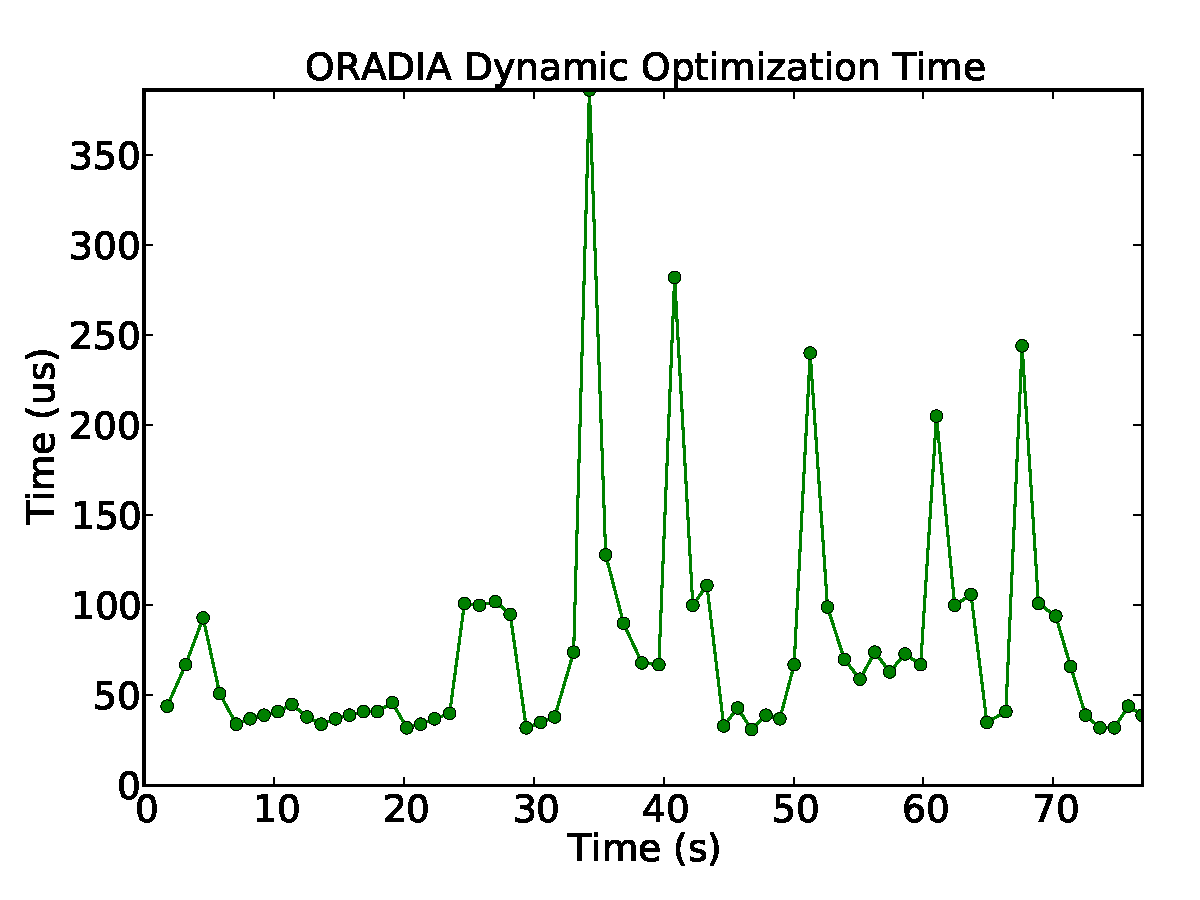
\includegraphics[bb=0 0 576 432,width=\columnwidth]{opt_time.pdf}
%%		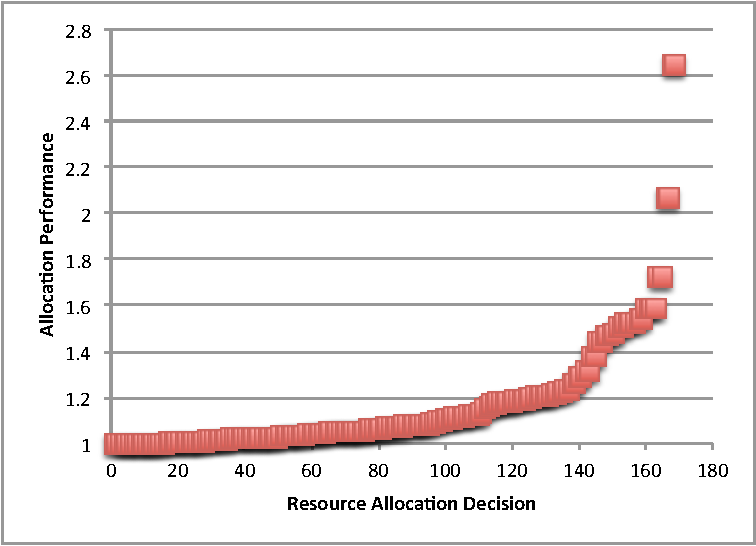
\includegraphics[width=.45\textwidth]{parsec_decision_points.pdf}
%		\caption{Performance of our penalty optimization algorithm}
%		\label{optimization_perf}
%	\end{center}
%\end{figure}


%Figure~\ref{optimization_perf} shows performance of the penalty optimization algorithm implemented in \tess.  

%For our video conferencing scenario the average runtime is \fix{x} and then worst case runtime is \fix{y}.  \fix{explain where the variance comes from}


\subsection{Resource allocation}

We follow the notation in \S 7.3 of Boyd et al. \cite{ADMM},
from which this material is taken almost verbatim.
We have $n$ resources and $N$ participants.
We let $x_i \in \reals^n_+$ denote the vector of resources 
that participant $i$ consumes.  
The (vector of) total resource consumption is then $x_1 + \cdots + x_N$;
for future use we let $z$ denote the average resource
usage per participant, \ie, the total divided by $N$.
Participant $i$ has a cost function $f_i:\reals^n \to \reals \cup
\{\infty\}$, where
$f_i$ is convex.  We let $f_i$ take on the value $+\infty$ to encode
constraints on the resource allocation.

The total cost function is
\[
f_1(x_1) + \cdots + f_N (x_N) + g(Nz),
\]
where $g: \reals^n \to \reals \cup \{+\infty\}$ is the cost
of consuming a total amount of resources (including any limits on total
available resources).
Note that the first $N$ terms are the costs associated with the
participants, and the last term is the cost of providing the total
resources.
The problem is to choose the allocations $x_i$ to minimize the total cost,
which is a convex optimization problem \cite{BoVa,ADMM}.

We will solve this problem using the \emph{sharing ADMM algorithm}
from \cite{ADMM}:
\begin{eqnarray*}
x_i^{k+1} &:=&  \argmin_{x_i} \left( f_i(x_i) + (\rho/2)
\|x_i-x_i^k+\overline x^k-z^k+u^k\|^2_2\right)\\
z^{k+1} &:=&  \argmin_{z} \left( g(Nz) + (N\rho/2)
\|z - u^k - \overline x^{k+1} \|_2^2 \right)\\
u^{k+1} &:=&  u^k + \overline x^{k+1}- z^{k+1}.
\end{eqnarray*}
Here $\rho>0$ is an algorithm parameter,
$k$ is the iteration number,
and $\overline x^k$ is the average of the consumption vectors
$x^k_1, \ldots, x^k_N$.
We interpret $x_i^k$ as the (proposed) resource consumption of 
participant $i$,
$z^k$ as the (proposed) average resource consumption,
and $u^k$ as a dual variable, all at iteration $k$.
This algorithm converges to an optimal allocation,
and $(1/\rho)u^k$ converges
to the optimal dual variables (prices) for the resources.

The $x$-update can be carried out in parallel, for $i=1, \ldots, N$.
Each participant, in each iteration, must minimize a function of the form
\[
f_i(x_i) + (\rho/2) \|x_i - v\|_2^2,
\]
\ie, each participant evaluates a proximal operator; see
\cite{ProxAlgs}.

The $z$-update step requires
gathering $x_i^{k+1}$ to form the averages, and then solving a problem
with $n$ variables.  This step is also a proximal evaluation.

After the $u$-update, the new value of $\overline x^{k+1}-
z^{k+1}+u^{k+1}$ is scattered to the subsystems.

\subsection{Excess latency minimization}

We now specialize to a latency minimization problem,
where the participants are processes and the participant costs 
are related to their latencies.

\subsubsection{Participants}

The latency (time delay) of each process depends on the 
resources allocated to the process.
Our model of the latency of process $i$ is
\[
l_i(x_i) = a_i + \sum_{j=1}^n (w_i)_j/(x_i)_j
\]
for $x_i >0$, and $+\infty$ otherwise, where $a_i \in \reals_+$ and 
$w_i \in \reals_{++}^n$ are given latency model parameters.
The participant cost is given by
\[
f_i(x_i) = \alpha_i (l_i(x_i) - t_i)_+,
\]
where $\alpha >0$ is a parameter and $t_i$ is a target latency.
Note that $l_i(x_i)-t_i$ is the excess latency.

We commment that the target latency in the cost function here is
probably not the actual target latency for our system, but rather
a target latency below which we do not impose a cost.  If the system
specification is for process $i$ to have (to the extent possible) latency
not exceeding $T_i$, then we might choose, for example, $t_i= 0.9T_i$.
In this case, there is no latency cost as long as the process latency is
less than the specification latency, with at least $10\%$ margin.

In each iteration of the sharing algorithm, 
we need to evaluate the proximal operator of $f_i$.
To simply notation, we drop the subscript $i$ and consider one
participant.
We need to minimize
\[
\alpha \left(a + \sum_{j=1}^n w_j/x_j - t\right)_+ + 
(\rho/2)\sum_{j=1}^n (x_j - v_j)^2
\]
over $x_j\geq 0$.
Note that we can combine $\alpha$ and $\rho$ (say, by dividing by 
$\alpha$) and we can combine $a$ and $t$.  So we now 
assume that $\alpha =1$ and $a=0$, with the understanding that
$\alpha$ and $a$ have been incorporated into $\rho$ and $t$.

We work out several cases.  First suppose that the excess latency
is negative.  
The first term above is zero and we must have $x=v$.  So $x=v$ is
the solution when $v>0$ and
\[
\sum_{j=1}^n w_j/v_j - t \leq 0.
\]

Now consider the case when the excess latency is positive.  In this case
we simply minimize
\[
\sum_{j=1}^n w_j/x_j +
(\rho/2)\sum_{j=1}^n (x_j - v_j)^2,
\]
which can be done for each $x_j$ separately.
Each $x_j$ must satisfy
\[
w_j/x_j^2  = \rho(x_j - v_j).
\]
This can be solved extremely quickly, using a bisection method, Newton's
method, or many others to find the unique (positive) 
values $x_j^\star$ that satisfy
the equation.
We then check if the resulting values of $x_j$ give nonnegative
excess latency, \ie, if 
\[
\sum_{j=1}^n w_j/x_j^\star - t  \geq 0.
\]
If so, we are done: $x^\star$ is the value of the proximal operator.

Finally, we consider the special case (which occurs often) when
the optimal values have zero excess latency, \ie,
\[
\sum_{j=1}^n w_j/x_j - t  = 0.
\]
The optimality condition in this case is that exists a $\theta \in [0,1]$
for which
\[
\theta w_j/x_j^2 = \rho(x_j - v_j)
\]
(along with the condition $\sum_{j=1}^n w_j/x_j - t  = 0$).
This we solve by bisection on $\theta$.  For each value of $\theta$,
we use the same method as above to find $x_j$.  We then check if
$\sum_{j=1}^n w_j/x_j - t  = 0$ is positive or negative.
If it is positive, we increase $\theta$; otherwise we decrease it.
(We could also apply a Newton method to solve the two equations for
$x_j$ and $\theta$.)

\paragraph{Summary.} 
We can write a little C code that computes the proximal operator
for each participant very fast.
A naive implementation will be fast; an optimized one (say,
in whcih we precompute the solution with a lookup table) will be very very
fast.

\subsubsection{Total resource cost}

We take the resource cost to have the form
\[
g(z) = \sum_{i=1}^n g_i(z_i).
\]
Here $g_i(z_i)$ is the cost of providing resource $i$ at level $z_i$.
A simple model is 
\[
g_i(z_i) = \left\{ \begin{array}{ll} 
c_i z_i & z_i \leq Z_i\\
+ \infty & z_i > Z_i ~\mbox{or}~z_i<0,
\end{array} \right.
\]
where $Z_i>0$ is the maximum available, and $c_i>0$ is the price for
resource $i$.
Since $g$ is separable, we can minimize over each resource 
separately; these are scalar problems.

We need to minimize 
\[
g_i(Nz_i)  +(N\rho/2)(z_i - v_i)^2
\]
over the (scalar) $z_i$. (Here $v_i = u^k_i + \overline x^{k+1}_i$.)
The solution is simple:
\[
    z_i = \max \{0, \min \{ v_i - c_i/\rho, Z_i/N\} \}.
\]
Note that $N$ drops out, but we need to scale the bound accordingly.
Also note that when the average $z_i = Z_i/N$, the total amount of
resource is $N z_i=Z_i$, meaning 
that resource $i$ is at its maximum possible level.

%\paragraph{Summary.} We can write a few lines of C code that carries out
%the $z$ update step.  It will be exceedingly fast.

\subsubsection{Total resource cost with free zone}
We model the resource cost in terms of energy consumed with a function 
of the form
\[
    g(z) = \lambda \left(\sum_{i=1}^n c_i z_i - b\right)_+,
\]
where $c_i>0$ represents the amount of energy consumed by
unit amount of resource~$i$, 
the constant~$b>0$ is a threshold below which power consumption is free,
and~$\lambda>0$ is the price charged for excess energy used
(or relative weight used to tradeoff between latency and energy).
We also impose lower and upper bounds on~$z$, \ie, $0\leq z_i\leq Z_i$
for $i=1,\ldots, n$.

To evaluate the proximal operator, we need to minimize
\[
    g(Nz) + \frac{N\rho}{2}\sum_{i=1}^n (z_i-v_i)^2,
\]
where $z$ is the averge resource vector, and
$v_i = u^k_i + \overline x^{k+1}_i$.
This is equivalent to
\[
\begin{array}{ll}
\mbox{minimize} &  \lambda\left(\sum_{i=1}^n c_i z_i - b/N\right)_+
     + (\rho/2)\sum_{i=1}^n (z_i-v_i)^2 \\
\mbox{subject to} & 0\leq z_i \leq Z_i/N, \quad i=1,\ldots,n.
\end{array}
\]
The solution can be obtained in a way similar to that used for evaluating 
the proximal operator of the latency penalty functions.

We work out several cases. 
First suppose that the excess energy is negative. 
The first term in the objective function is zero. 
So the solution is
\[
    z_i = \max\{0, \min\{v_i, Z_i/N\}\}, \quad i=1,\ldots, n
\]
provided that
\[
    \sum_{i=1}^n c_i z_i - b/N \leq 0.
\]

Next we consider the case when the excess energy is positive.
In this case, we simply minimize
\[
    \lambda \left(\sum_{i=1}^n c_i z_i - b/N \right) 
    + (\rho/2)\sum_{i=1}^n (z_i-v_i)^2,
\]
which can be solved for each $z_i$ separately and the solutions are
\[
    z_i = \max\{0, \min\{v_i - \lambda c_i/\rho, Z_i/N\}\}, \quad i=1,\ldots, n.
\]
We then need to check
\[
    \sum_{i=1}^n c_i z_i - b/N \geq 0.
\]
If so, we are done.

Finally we consider the case when the optimal allocations have zero excess
enerty, \ie,
\[
    \sum_{i=1}^n c_i z_i - b/N = 0.
\]
The solution takes the form
\[
    z_i = \max\{0, \min\{v_i - \theta c_i/\rho, Z_i/N\}\}, \quad i=1,\ldots, n.
\]
where $0\leq\theta\leq\lambda$.
We can do a bisection on $\theta$ to make the solution satisfy
$\sum_{i=1}^n c_i z_i-b/N=0$.
Basically, if the excess energy is positive, then we increase~$\theta$;
otherwise we decrease it.




\subsubsection{Smoothing regularization}

Suppose we need to do resource allocation repeatedly over time.
We can add a term of the form
\[
\mu \| x_i - x_i^\mathrm{prev}\|_1,
\]
where $\mu > 0$ is a parameter, to the latency cost function.
This adds a cost for changing the resource allocation from its
previous value.
The larger $\mu$ is, the less frequently the resource allocations change
over time (which comes at the cost of higher objective cost).
As an extension, we can have different values of $\mu_i$ for each
resource; this allows some resource levels to be adjusted more often than
others.

The addition of smoothing regularization would require a few 
changes to the proximal operator evaluation described above.

\subsection{Real-time resource allocation}

Here we describe how the sharing algorithm is used in a real-time 
resource allocation system.
Resources are (possibly) re-allocated in time epochs.
In each time epoch, we (possibly) 
(re-)estimate the latency model parameters $a_i$, $w_i$, and
obtain (possibly) updated values for the resource usage cost 
parameters $c_i$ and $Z_i$.
These new values are used for the next round of sharing algorithm iteration,
starting from the values in the previous time epoch.  (This is called
\emph{warm start}.
The converged values are then used for the allocations in the 
current epoch.

\subsection{implementation details}

\subsubsection{Stopping criteria}
Here we describe a stopping criterion that is similar to the one
in \S3.3 of \cite{ADMM} applied the resource allocatoin problem.

For our resource allocation problem, the primal residuals at iteration~$k$ are
\[
    r_i^k = x_i^k - z_i^k, \quad i=1,\ldots,N,
\]
and the dual residuals are
\[
    s_i^k = \rho (z_i^{k-1}-z_i^{k}), \quad i=1,\ldots,N.
\]
Here $z_i$ for $i=1,\ldots, N$ are the variables that were eliminated
to simplify the $z$-update in the sharing problem 
(see \S7.3 of \cite{ADMM}).
The variable~$z$ in the  simplified update is actually 
their average $\overline z=(1/N)\sum_{i=1}^N z_i$.
Based on the derivation in \cite[\S7.3]{ADMM}, 
\[
    z_i^k = x_i^k -\overline x^k + \overline z^k , \quad i=1,\ldots,N.
\]
Therefore we have
\[
    r_i^k = x_i^k - z_i^k = \overline x^k - \overline z^k, \quad i=1,\ldots,N,
\]
\ie, the primal residuals for the processes are the same as the average
primal residue.
The dual residuals become
\begin{eqnarray*}
    s_i^k &=& \rho(z_i^{k-1} - z_i^k) \\
    &=&\rho\bigl( (x_i^{k-1}-x_i^k) +(\overline x^k-\overline z^k)
    -(\overline x^{k-1} - \overline z^{k-1})\bigr)\\
    &=& \rho\bigl( (x_i^{k-1}-x_i^k) + r^k - r^{k-1} \bigr),
    \quad i=1,\ldots, N.
\end{eqnarray*}
So the dual residuals are different for different processes.

The following termination criterion is similar to the one proposed in
\cite[\S3.3]{ADMM}:
\begin{eqnarray*}
\|r^k\|_2 = \|\overline x^k - \overline z^k\|_2 &\leq& \epsilon^\mathrm{pri},\\
\max \{\|s_1^k\|_2,\ldots,\|s_N^k\|_2 \} &\leq& \epsilon^\mathrm{dual},
\end{eqnarray*}
with
\begin{eqnarray*}
\epsilon^\mathrm{pri} &=& \sqrt{n}\epsilon^\mathrm{abs} + \epsilon^\mathrm{rel}
    \max\{\|x_1\|_2,\ldots,\|x_N\|_2,\|z_1\|_2,\ldots,\|z_N\|_2\} ,\\
\epsilon^\mathrm{dual} &=& \sqrt{n}\epsilon^\mathrm{abs} +\epsilon^\mathrm{rel}
    \rho\|u^k\|_2.
\end{eqnarray*}


Since the computation involved in the above stopping criterion are 
rather heavy, and we also experimented with simplified conditions.
In particular, we tried the following conditions 
which only uses the average vectors:
\begin{eqnarray*}
\|r^k\|_2=\|\overline x^k - \overline z^k\|_2 
&\leq& \sqrt{n}\epsilon^\mathrm{abs}+\epsilon^\mathrm{rel}\|\overline z^k\|_2,\\
\|s^k\|_2 = \rho(\overline z^{k-1}-\overline z^k\|_2)
&\leq& \sqrt{n}\epsilon^\mathrm{abs} +\epsilon^\mathrm{rel}\rho \|u^k\|_2 .
\end{eqnarray*}
Basically we simplified the calculation of $\epsilon^\mathrm{pri}$ and
the dual residual, while leave the calculation of primal residual and
$\epsilon^\mathrm{dual}$ unchanged.

Figure~\ref{fig:residual-e} shows both the accurate calculations and their
simplified counterparts.
We see that the simple primal $\epsilon^\mathrm{pri}$ is slightly smaller
than the more accurate calculation, making primal residual a little harder to
satisfy the termination condition. 
On the other hand, the simple dual residual calculation is smaller than
the accurate dual residual calculation, making thedual residual easier to
satisfy the termination condition.
Figure~\ref{fig:allocation-e} illustrate the optimal resource allocation 
and resulting latency for each of the processes.

It looks that the simplified stopping criterion is effective and 
sufficient.
However, when we vary the parameters in the resource allocation problem, 
the simple conditions may breakdown.
Figure~\ref{fig:residual-c} and~\ref{fig:allocation-c} 
plot the same quantities but in the case of cheap energy (meaning that
price $\lambda$ in the total resource cost function is small).
In this case, the total resouces allocated all reach their bounds, 
and most of the process latency are within their deadlines.
Notice that the simplified dual residual becomes exactly zero 
(discontinued in the right plot of Figure~\ref{fig:residual-c}) 
after 10 iterations.
The reason is that since the enerygy is cheap, the resource allocations 
reach their bounds easily,
so the simple dual residual $\|s^k\|_2=\rho\|z^{k}-z^{k+1}\|_2=0$ 
become zero quickly, therefore can \emph{not} serve as a stopping criterion.

In our implementation, we use the simplfied calculation of 
$\epsilon^\mathrm{pri}$,
but do not simplify the calculation of the dual residual.

\begin{figure}[th]
\centering
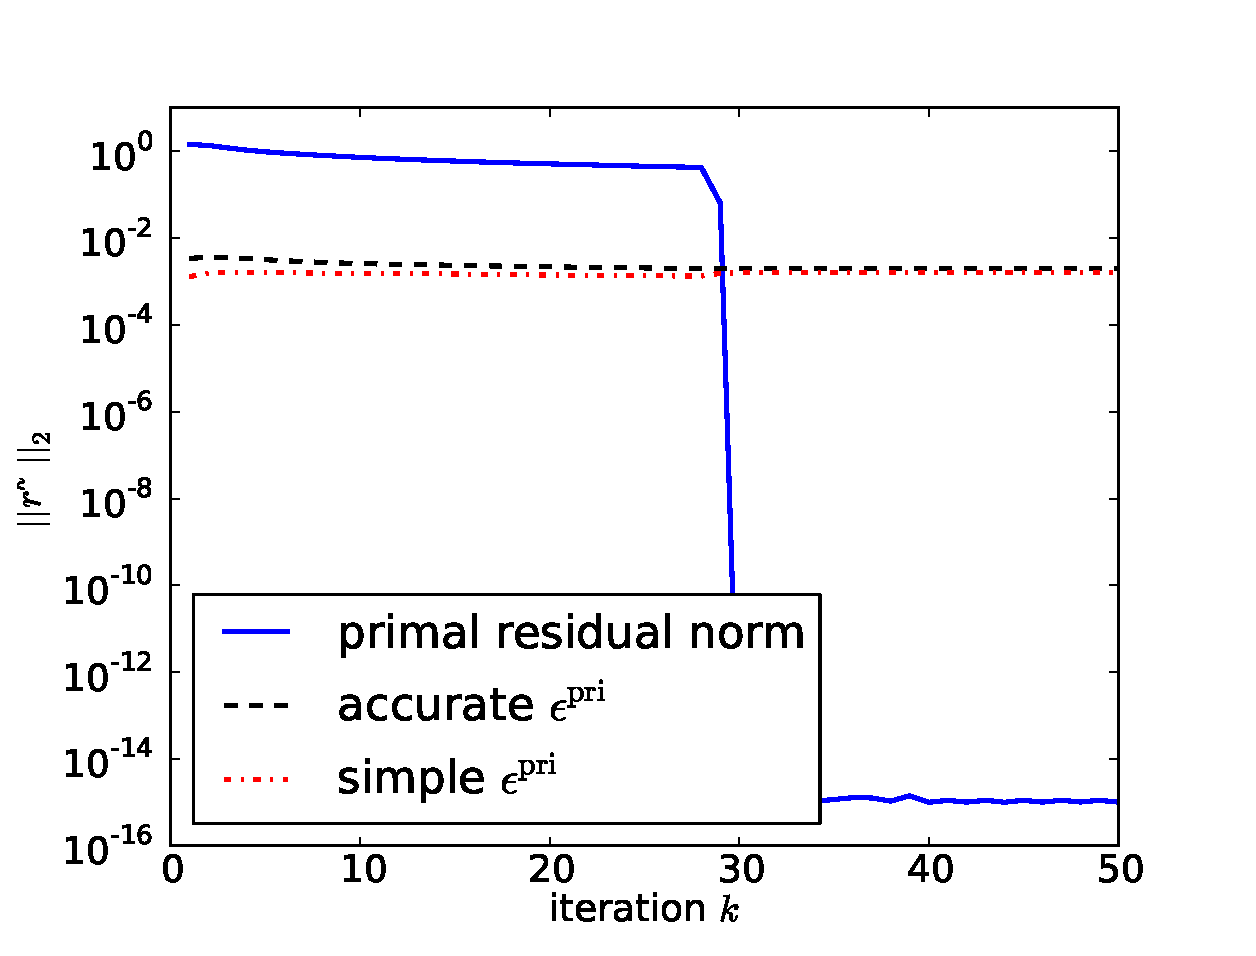
\includegraphics[width=0.49\textwidth]{figures/test_primal_e.eps}
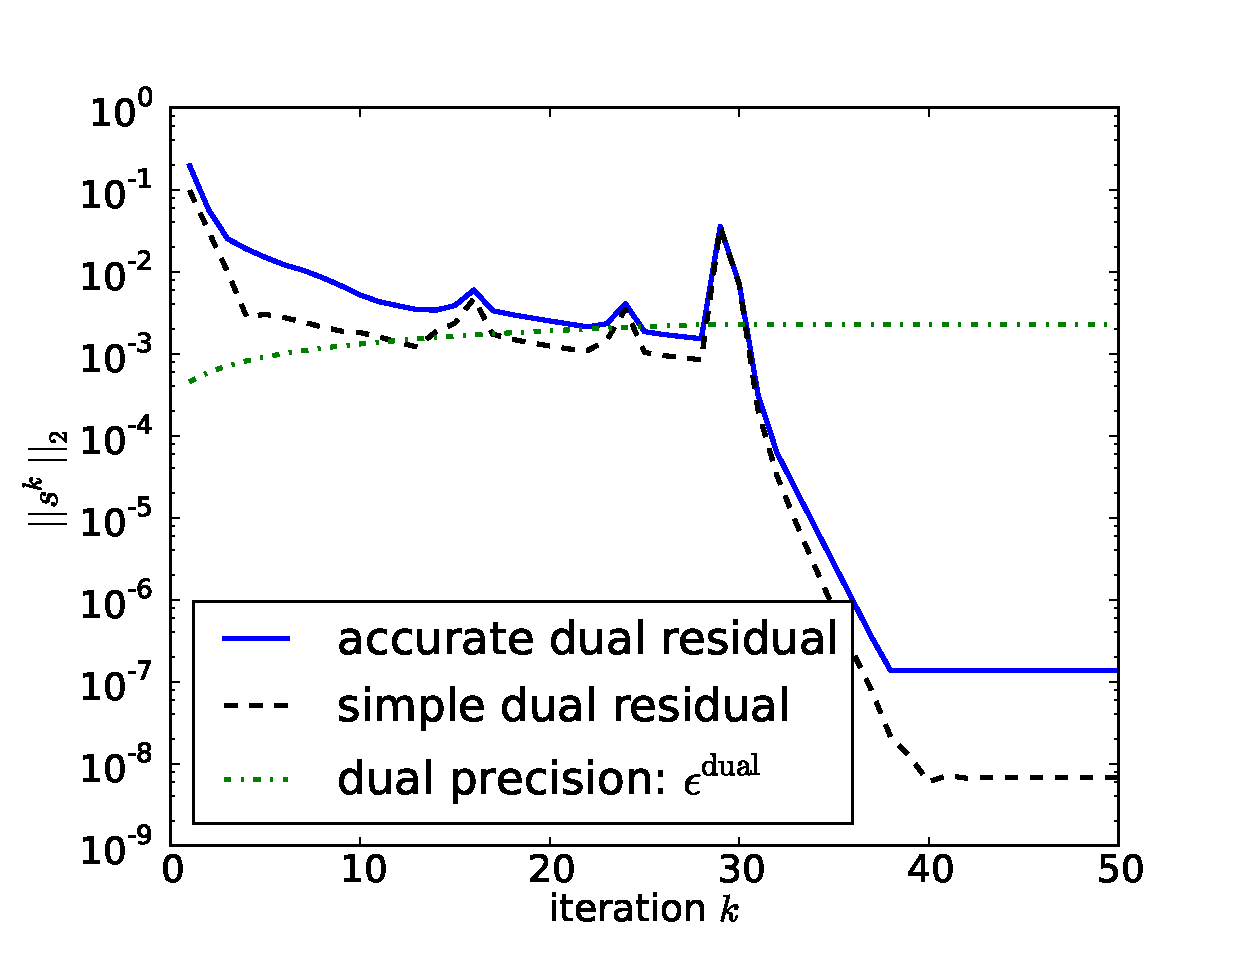
\includegraphics[width=0.49\textwidth]{figures/test_dual_e.eps}
\caption{Progress of reducing primal and dual residual norms in ADMM.
    This is the case of expensive energy, notice that the simple dual
residual often work as well as the accurate dual residual. Since
the resource allocations are not reaching their bounds, so the simple
dual residual $\|s^k\|_2=\rho\|z^{k}-z^{k+1}\|_2$ converges to zero 
only asymptotically, and can serve as a stopping criterion.}
\label{fig:residual-e}
\end{figure}

\begin{figure}[th]
\centering
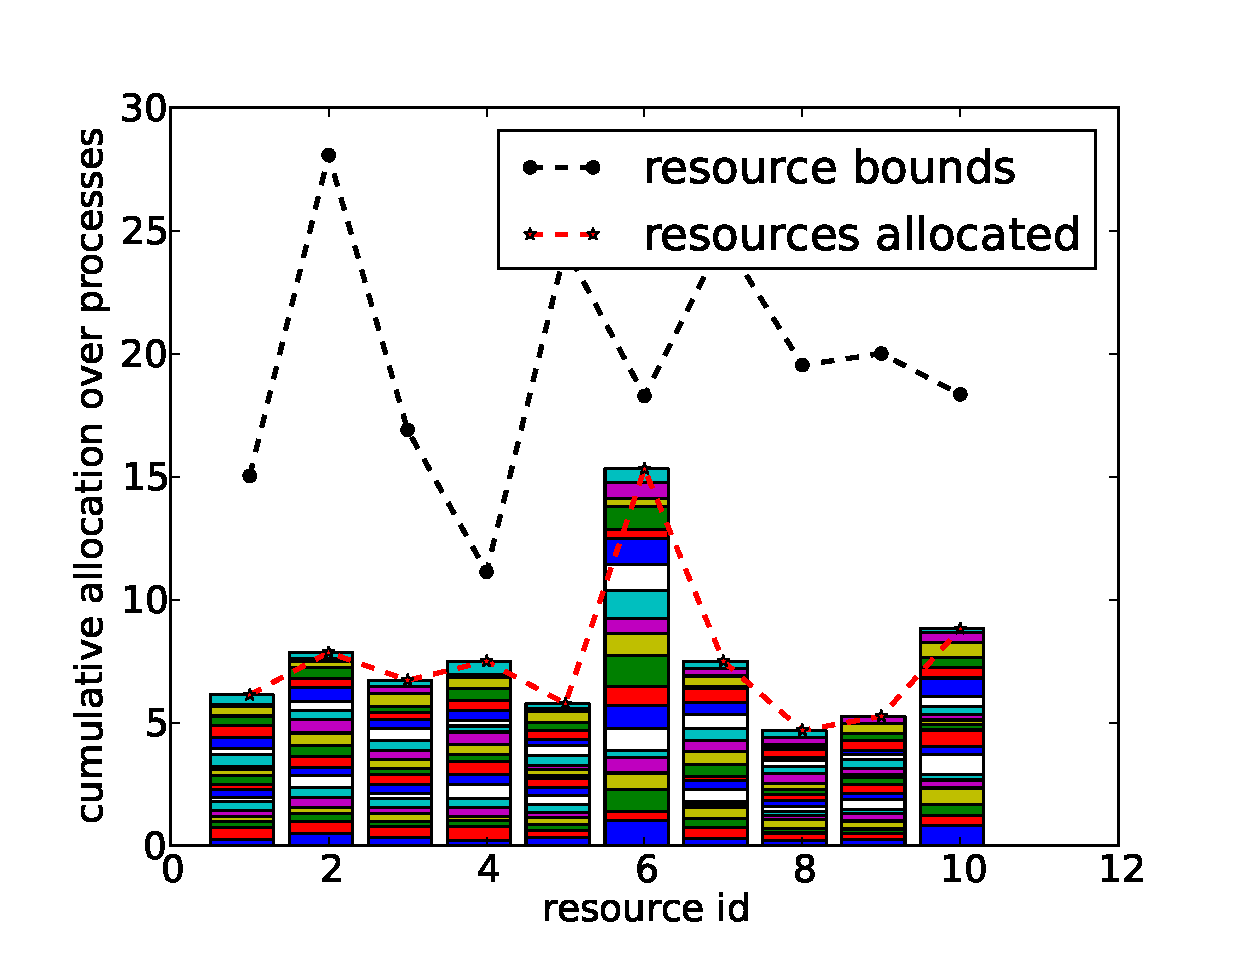
\includegraphics[width=0.49\textwidth]{figures/test_resource_e.eps}
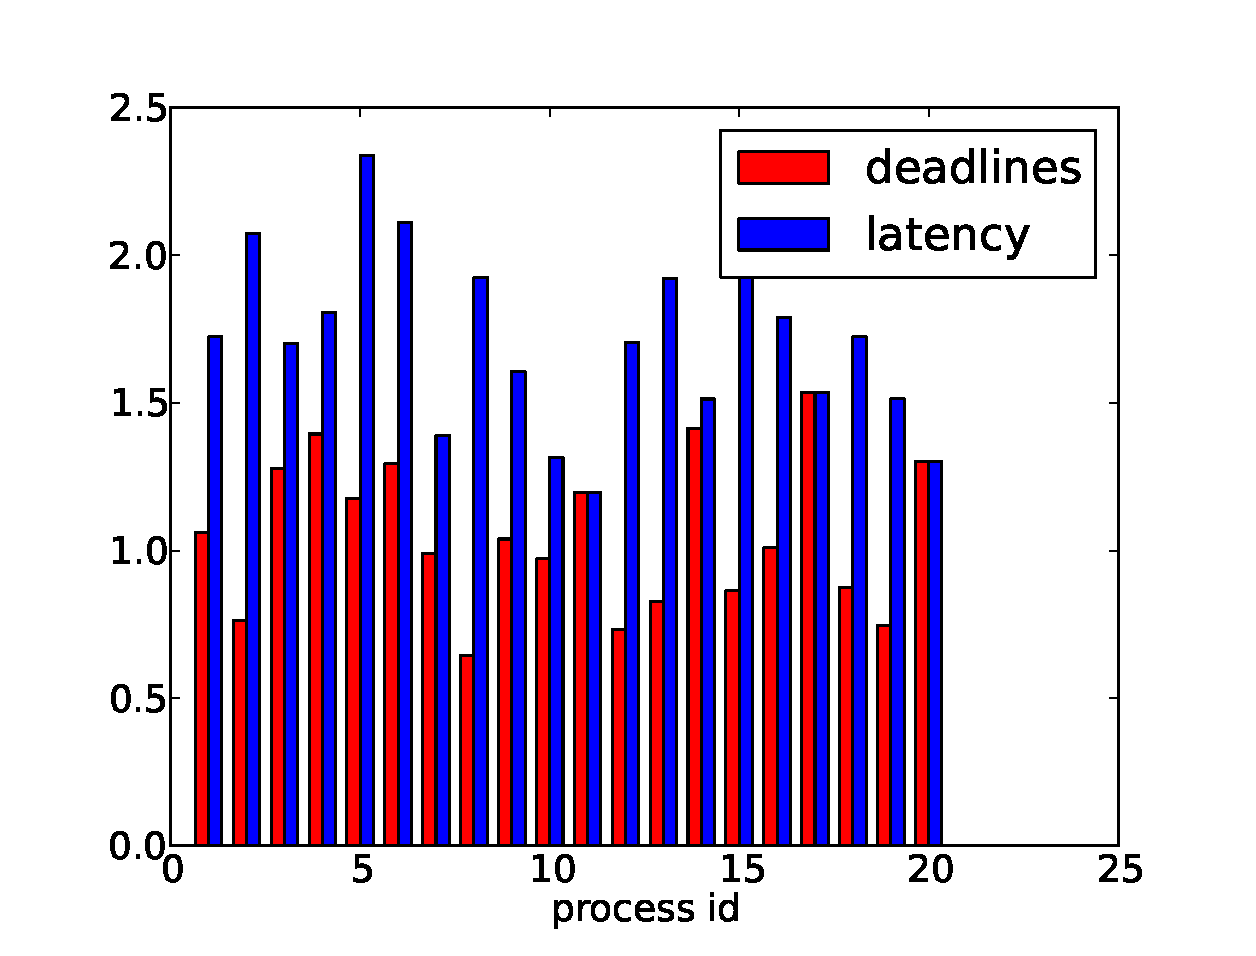
\includegraphics[width=0.49\textwidth]{figures/test_latency_e.eps}
\caption{Visualization of optimal resource allocation (left) and 
    resulting latency for each process (right).
    There are $n=10$ resources and $N=20$ processes.
    This is the case of expensive energy, so the total resouces allocated
    are mostly well below their bounds, but the process latency are mostly
exceeding the deadlines.}
\label{fig:allocation-e}
\end{figure}


\begin{figure}[th]
\centering
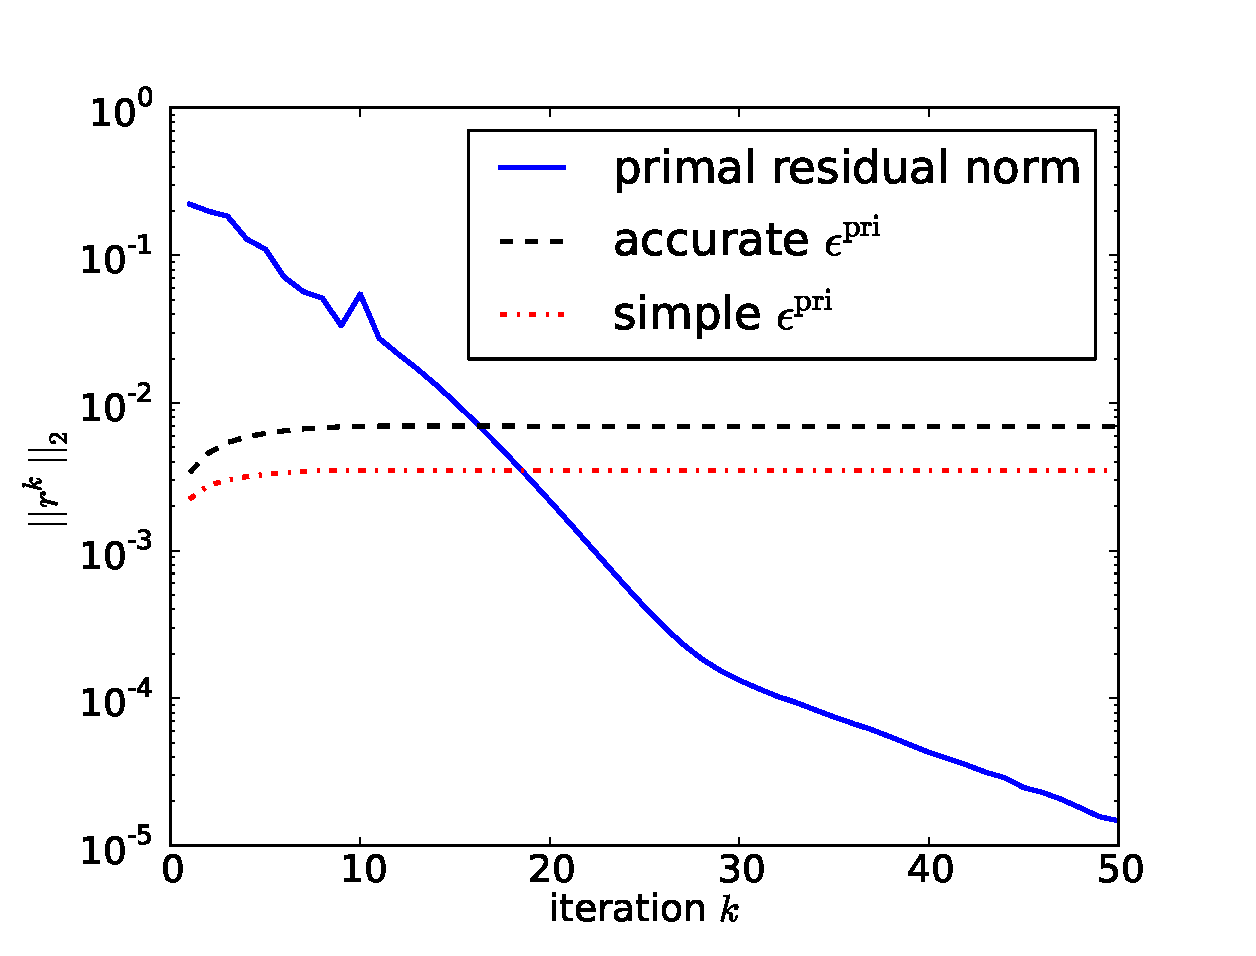
\includegraphics[width=0.49\textwidth]{figures/test_primal_c.eps}
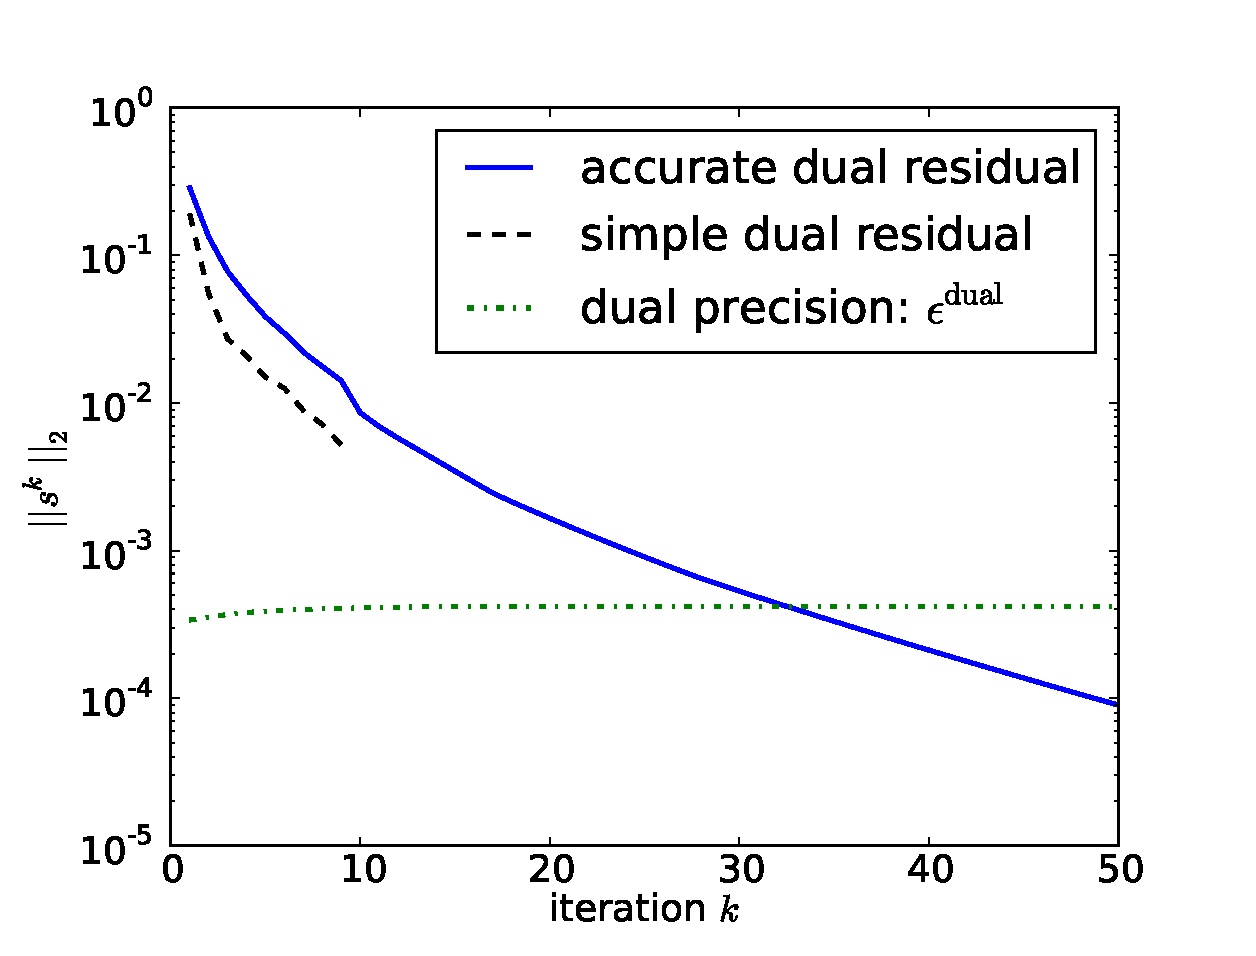
\includegraphics[width=0.49\textwidth]{figures/test_dual_c.eps}
\caption{Progress of reducing primal and dual residual norms in ADMM.
    This is the case of cheap energy, notice that the simple dual
residual becomes exactly zero (discontinued in the plot) after 10 iterations, 
Since the enerygy is cheap, the resource allocations reach their bounds easily,
so the simple dual residual $\|s^k\|_2=\rho\|z^{k}-z^{k+1}\|_2=0$ 
become zero quickly, therefore can \emph{not} serve as a stopping criterion.}
\label{fig:residual-c}
\end{figure}

\begin{figure}[th]
\centering
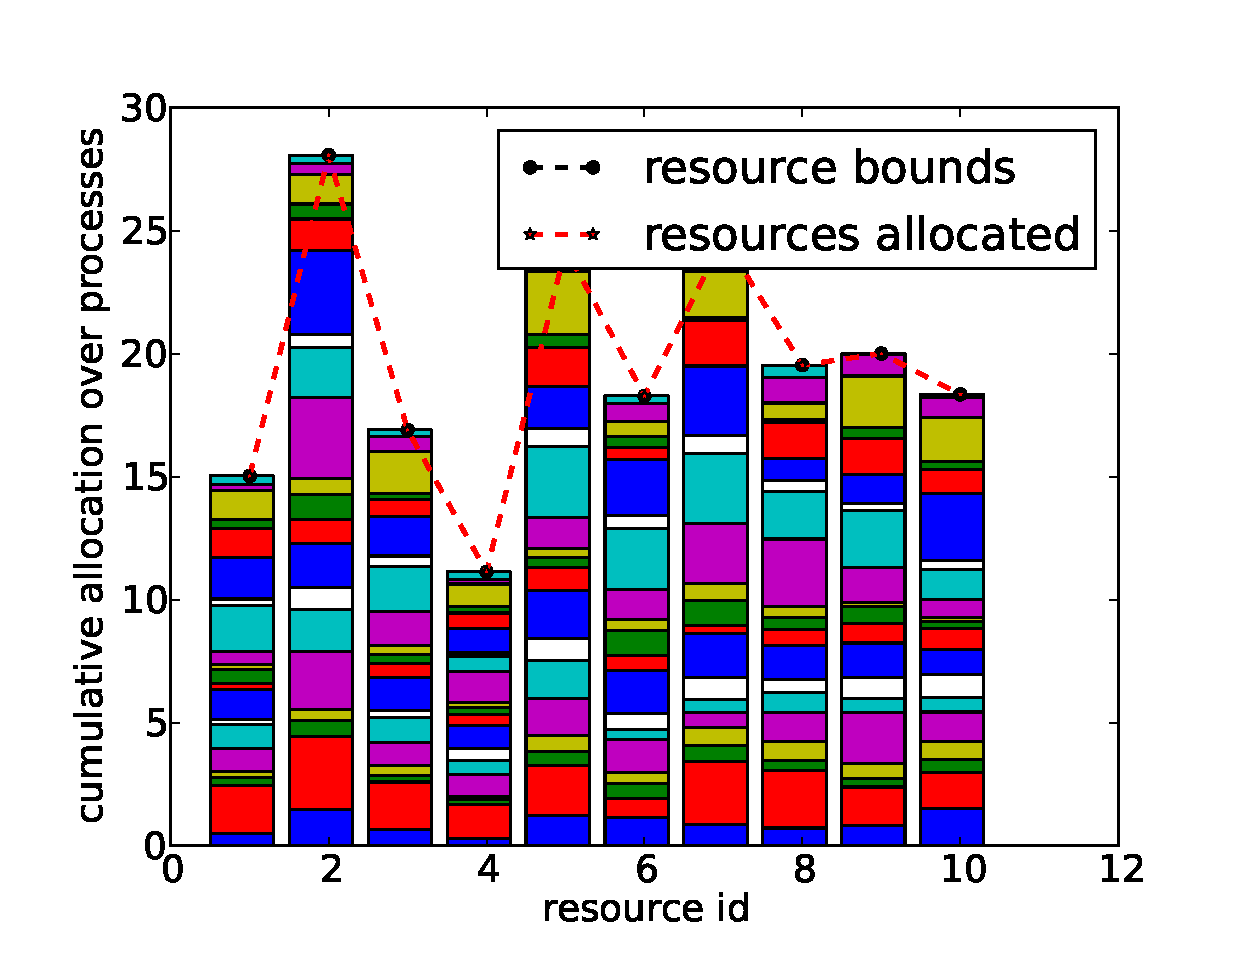
\includegraphics[width=0.49\textwidth]{figures/test_resource_c.eps}
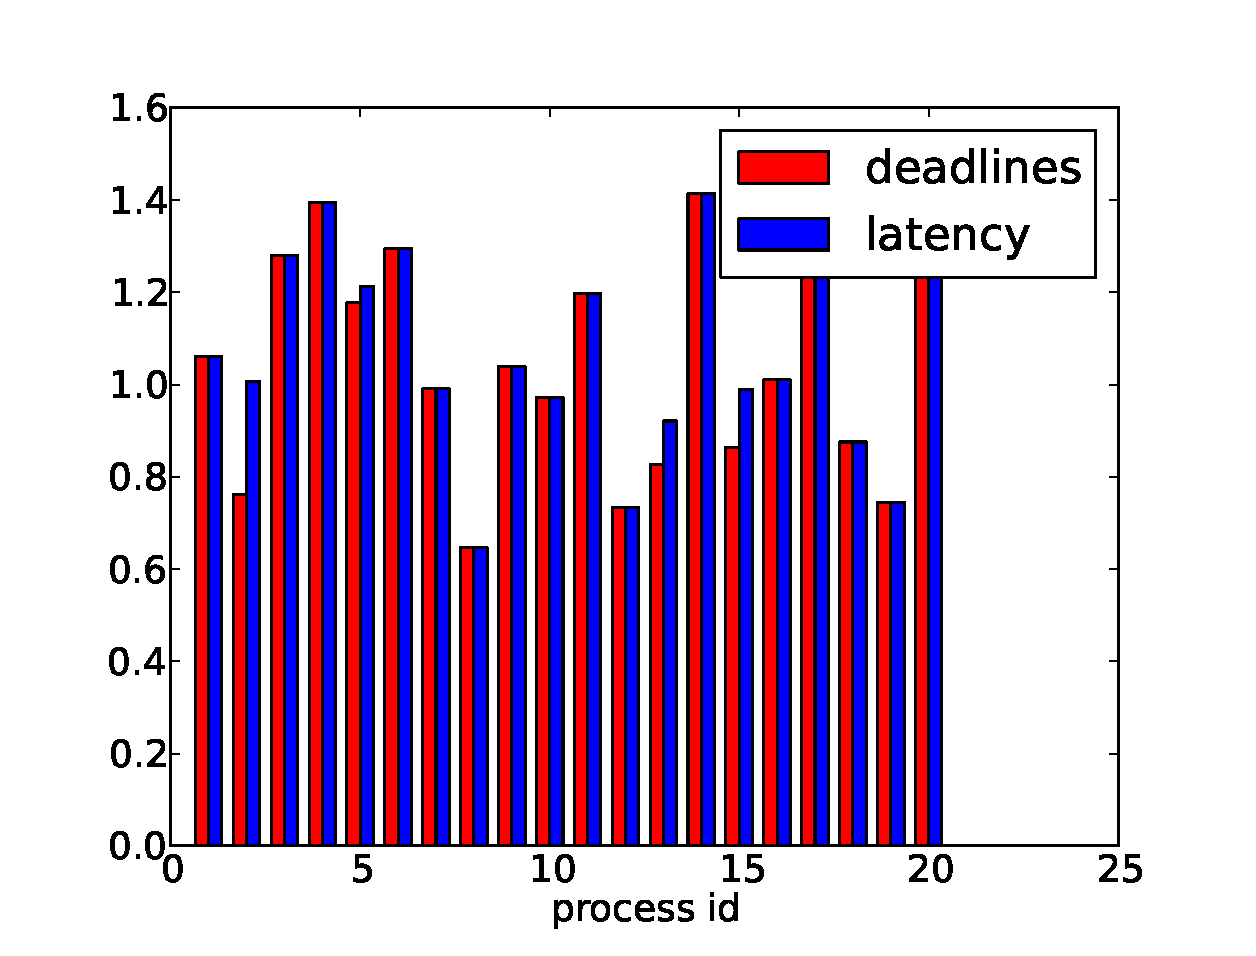
\includegraphics[width=0.49\textwidth]{figures/test_latency_c.eps}
\caption{Visualization of optimal resource allocation (left) and 
    resulting latency for each process (right).
    There are $n=10$ resources and $N=20$ processes.
    This is the case of cheap energy, so the total resouces allocated
    all reach their bounds, and most of the process latency are 
within their deadlines.}
\label{fig:allocation-c}
\end{figure}

\section{Summary}

